% 16-annexes.tex — Annexes (hors des ≈ 75 pages du corps).

\chapter{Instruments d'évaluation}
\label{ann:instruments}

\begin{arediger}{selon besoin}
Test conceptuel complet, questionnaire de perception, grille d'observation.
\end{arediger}

\chapter{Fichier de règles \fichier{CLAUDE.md}}
\label{ann:claude}

\begin{arediger}{2 à 3 pages}
Reproduire la version finale du fichier de règles du dépôt (en anglais, tel
quel) avec une courte introduction.
\end{arediger}

\chapter{Galerie des simulations}
\label{ann:galerie}

\begin{figure}[H]
  \centering
  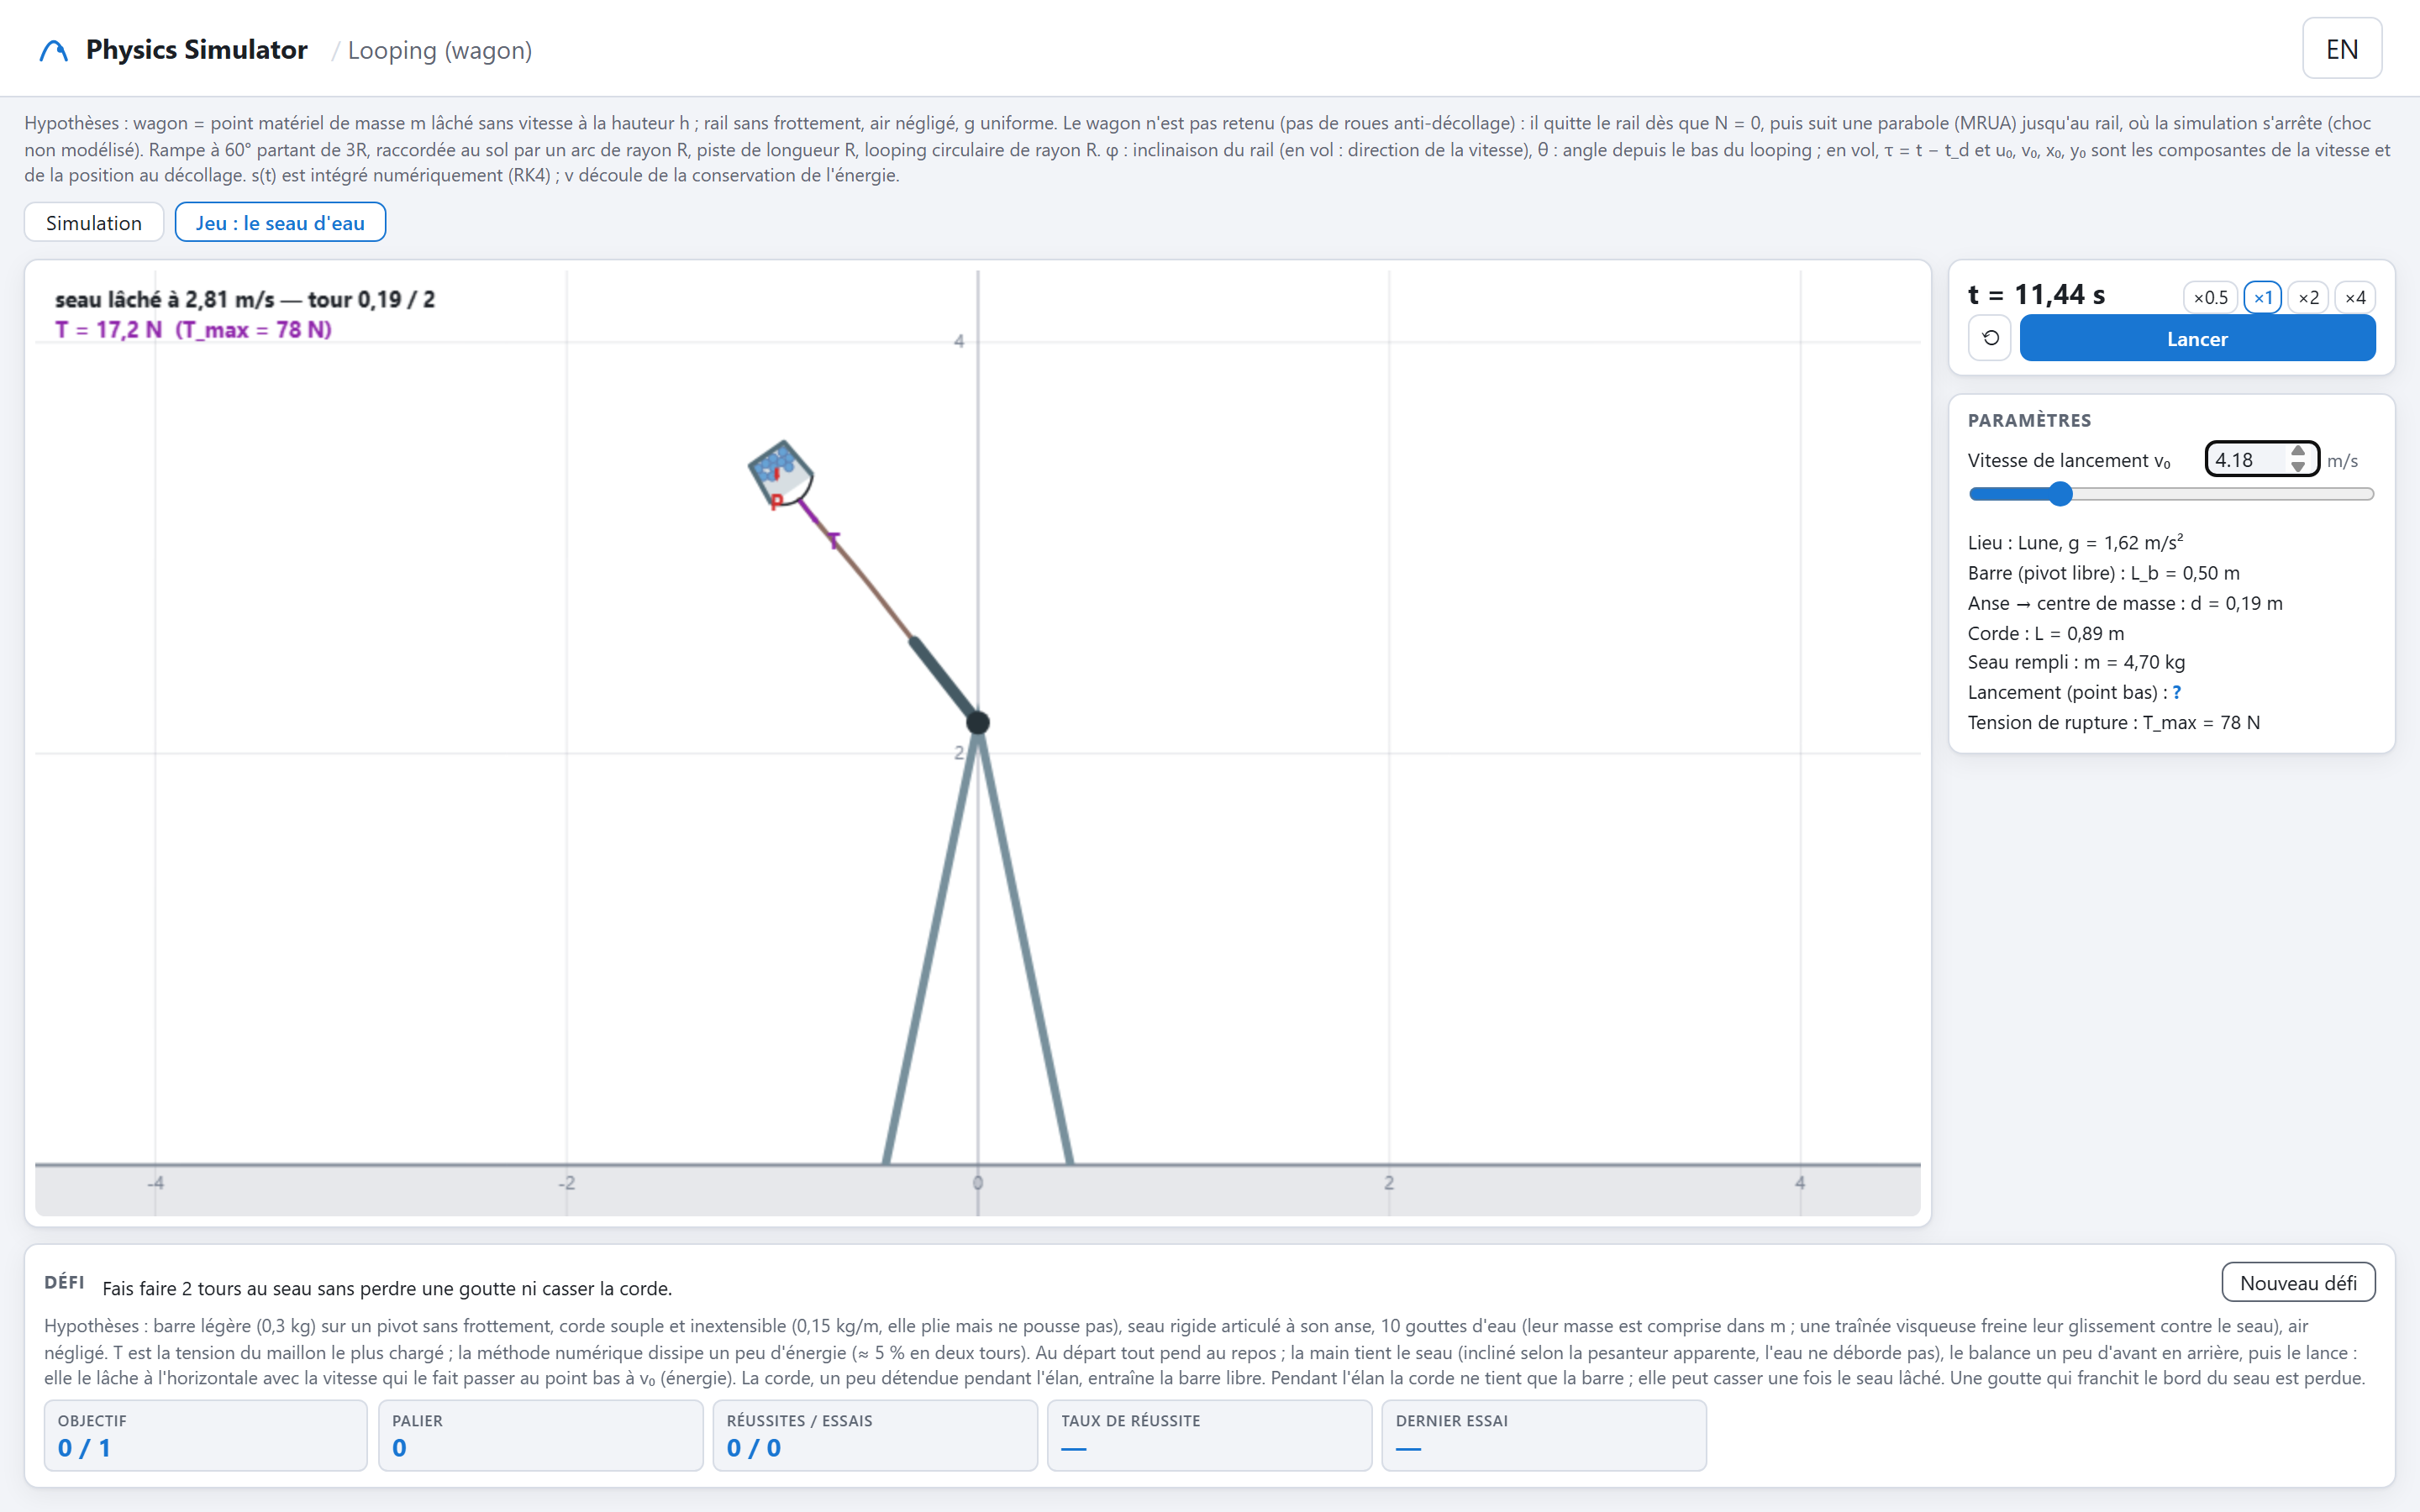
\includegraphics[width=\linewidth]{figures/captures/jeu-ecran-complet.png}
  \caption{Mode jeu du looping sur un écran de \(1440 \times 900\) pixels : scène
    fixe, réglage de la seule grandeur libre et données du défi à droite, panneau
    des statistiques et hypothèses en bas.}
\end{figure}

\begin{arediger}{2 à 4 pages}
Une capture par exercice (tir parabolique, pendule, MCU, looping
historique), avec une légende d'une ligne. Les captures se régénèrent avec
\fichier{outils/captures.cjs} (à étendre aux autres pages).
\end{arediger}
